
\section{Experimental Results}
I had tried my project on different server also i.e Experimental Server here. I had tried it on both ubuntu 14.04 and 15.10. It works fine on both versions.\\
Below is one of the experimental result.\\
\begin{figure}[!ht]
	\centering
	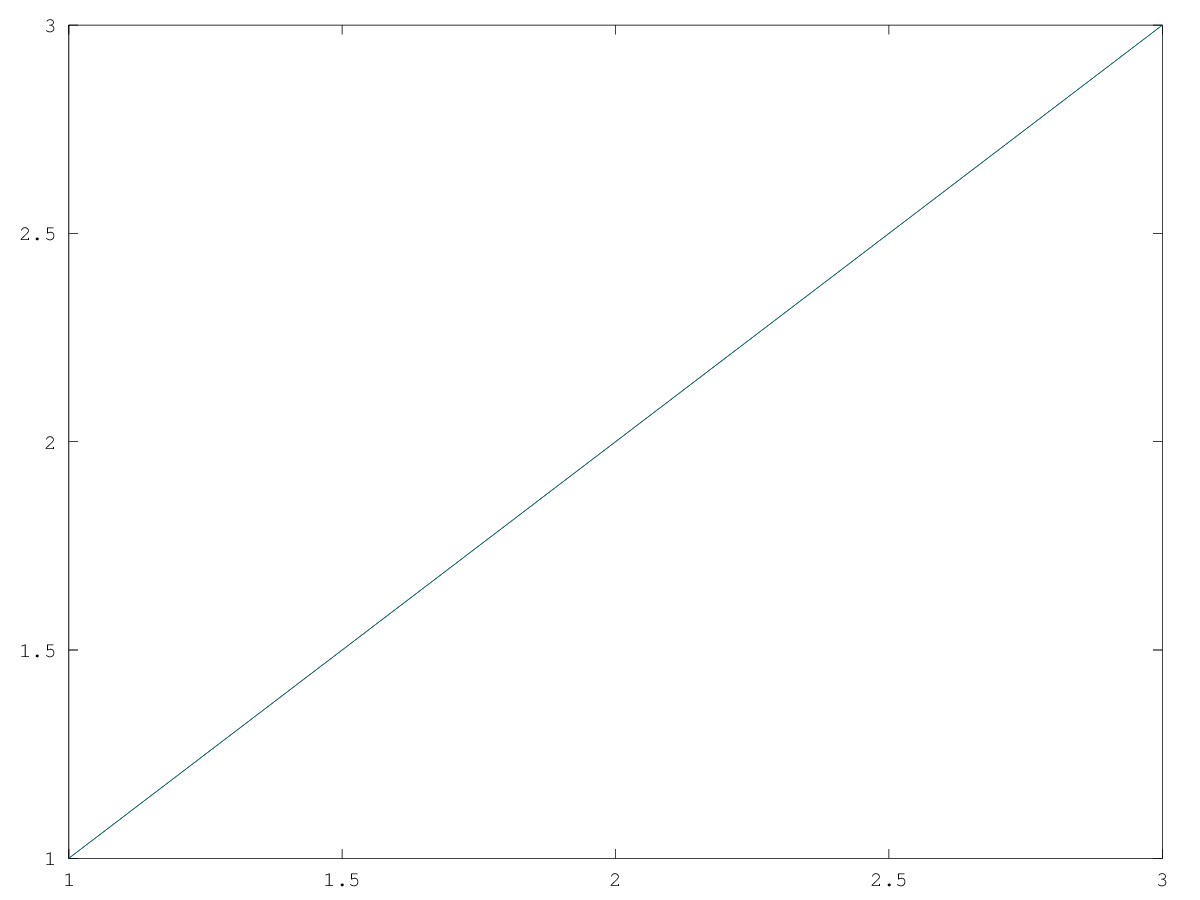
\includegraphics[width=0.7\textwidth]{input/images/plot1.png}                
	\caption{Graph Plotted}
	\hspace{-1.5em}
\end{figure}\\
You may refer to my blogs also for detailed information.\\
Here is the url: \\
https://deepti96.wordpress.com/ \\\\
The interface of Web-Octave looks like this but can be changed using CSS file.
\begin{figure}[!ht]
	\centering
	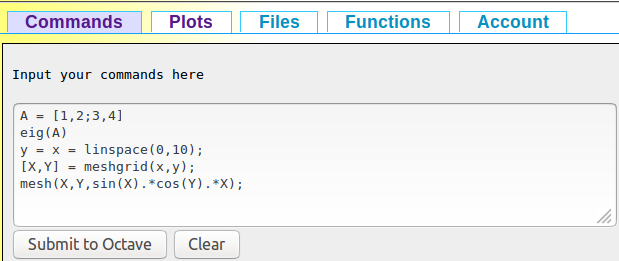
\includegraphics[width=0.7\textwidth]{input/images/p.png}                
	\caption{Code}
	\hspace{-1.5em}
\end{figure}\\\\
Output of above code is: \\
\begin{figure}[!ht]
	\centering
	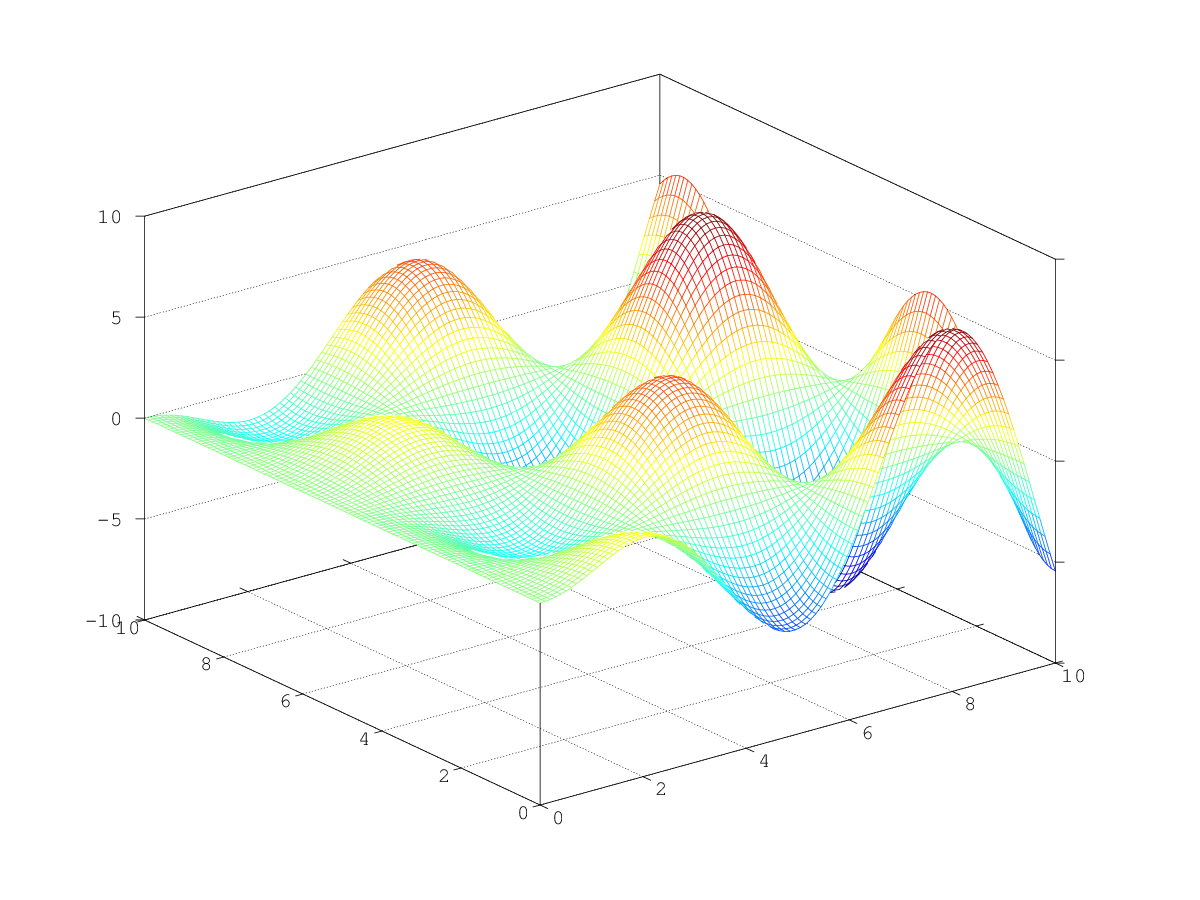
\includegraphics[width=0.7\textwidth]{input/images/plot2.png}                
	\caption{Output}
	\hspace{-1.5em}
\end{figure}\\
\subsection{Testing}
Testing a program consists of providing the program with a set of test inputs (or test cases) and
observing if the program behaves as expected. If the program fails to behave as expected, then the
conditions under which failure occurs are noted for later debugging and correction. \\
This software had been taken through rigorous test to fully found potential causes of error and system failure
and full focus have been given to cover all possible exceptions that can 
occur and cause failure of the software.\\
As this software is based on intensive background process it have been taken care that 
if correct input and email address are given then processing of user job can even continue or a least automatically 
restart even after server shuts down or even crash.

\begin{table}[h]
\centering
\begin{tabular}{ ||c|c|| }
\hline
 \multicolumn{2}{||c||}{Overview of Octave versions} \\
 \hline
 Date & Publication Title \\ [0.5ex] 
 \hline \hline
	September 1999 & Octave framework 1.0 \\ \hline
	September 2001 & Octave framework 2.0 \\ \hline
	December 2001 & Octave criteria 2.0\\ \hline
	September 2003 & Octave-S v0.9 \\ \hline
	March 2005 & Octave-S v1.0 \\ \hline
	June 2007 & Octave 3.x\\ \hline
        March 2016 &  Octave 4.0.1        \\ \hline
	July 2016 & Octave 4.0.3 \\ [1ex]
 \hline
\end{tabular}
\caption{Octave Release}
\label{table2}
\end{table}

\begin{table}[h]
\centering
\resizebox{\textwidth}{!}{\begin{tabular}{ |c|c|c|c| }
\hline
 \multicolumn{4}{|c|}{Test cases for main page(index.html) } \\[0.5ex]
 \hline
 Input & Desired Output & Actual Output & Status \\ [0.5ex] 
 \hline \hline
 Inputs range exceeds & Alert user,Don't proceed & Alert user,Don't proceed. & Pass\\ \hline
 Incomplete Command & Alert user about range. Don't proceed & Alert user about range. Don't proceed & Pass\\ \hline
 PNG selected: No & Error & Don't proceed & Pass\\ \hline
 Session: Yes & Show email field after Submit & Show email field after Submit & Pass\\ \hline
 Help pressed  & Show Detailed user help & Show Detailed user help  & Pass\\ \hline
 
\end{tabular}}
\caption{Computational Analysis}
\label{table3}
\end{table}
\begin{table}[h]
\centering
\resizebox{\textwidth}{!}{
\begin{tabular}{ |c|c|c|c| }
\hline
 \multicolumn{4}{|c|}{Test cases for possible source of problems } \\[0.5ex]
 \hline
  Input & Desired Output & Actual Output & Status \\ [0.5ex] 
 \hline \hline 
 URL refreshed & Send to homepage & Send to homepage & Pass\\ \hline
 server stops or rebooted & Start processing interrupted requests & Start processing interrupted requests & Pass\\ \hline
\end{tabular}}



\caption{Test case (general)}
\label{table}
\end{table}
 
 
 

